\documentclass[11pt]{article}
 
\usepackage[margin=1in]{geometry} 
\usepackage{amsmath,amsthm,amssymb}
\usepackage{graphicx} 


\newcommand{\N}{\mathbb{N}}
\newcommand{\Z}{\mathbb{Z}}
 
\newenvironment{problem}[2][Problem]{\begin{trivlist}
\item[\hskip \labelsep {\bfseries #1}\hskip \labelsep {\bfseries #2.}]}{\end{trivlist}}
\newenvironment{lemma}[2][Lemma]{\begin{trivlist}
\item[\hskip \labelsep {\bfseries #1}\hskip \labelsep {\bfseries #2.}]}{\end{trivlist}}
\newenvironment{exercise}[2][Exercise]{\begin{trivlist}
\item[\hskip \labelsep {\bfseries #1}\hskip \labelsep {\bfseries #2.}]}{\end{trivlist}}

\newenvironment{question}[2][Question]{\begin{trivlist}
\item[\hskip \labelsep {\bfseries #1}\hskip \labelsep {\bfseries #2.}]}{\end{trivlist}}
\newenvironment{corollary}[2][Corollary]{\begin{trivlist}
\item[\hskip \labelsep {\bfseries #1}\hskip \labelsep {\bfseries #2.}]}{\end{trivlist}}

\usepackage{indentfirst}
\linespread{1.2}     % 调整间距
\setlength{\parindent}{0pt}

\begin{document}

 
% --------------------------------------------------------------
%                         Start here
% --------------------------------------------------------------
 
\title{Homework 2 DS-GA 1002 }%replace X with the appropriate number
\author{Yuhao Zhao\\ %replace with your name
N17578783} %if necessary, replace with your course title
 
\maketitle
\begin{problem}{1}
\end{problem}
(a) The position of spider can be modeled By F(X,Y). X is the horizontal position and Y is the height position. \\
Since we know that the spider stays twice the time under the painting area, and is uniformly distributed both inside and outside the painting area.\\
We have $P((X,Y)\in paint) = 2 P((X,Y)\notin paint )$\\
Let $
f_{X,Y}(x,y)  =
\begin{cases}
	c   \hspace{2in}  (x,y) \in [4,6] \times [6,8] \\
	d  \hspace{2in}  otherwise
\end{cases}
$\\
Then we have $c \times 4 = 2\times d\times 96$ and $4c = 192d, c = \frac{1}{6}, d = \frac{1}{288}$ \\
Therefore\\
$f_{X,Y}(x,y)$  =
$\begin{cases}
\frac{1}{6}   \hspace{2in} (x,y) \in [4,6] \times [6,8] \\
\frac{1}{288}  \hspace{2in}  otherwise
\end{cases}$\\

(b)\\
 (i) For $y \in [0,6], F(Y) = P(Y \in [0,y]) = \int_{0}^{y} \int_{0}^{10}  f_{X,Y}{(u,v)} du dv =  \int_{0}^{y} \int_{0}^{10}  \frac{1}{288}dudv = \frac{10}{288} y$,\\
the pdf is $\frac{dF}{dy} = \frac{10}{288} $\\
(ii) For $y \in [6,8],F(Y) = P(Y \in [6,y])+P(Y\in [0,6]) = \int_{6}^{y} \int_{0}^{10}  f_{X,Y}{(u,v)} du dv + \frac{60}{288}$\\
$  \int_{6}^{y} \int_{0}^{10}  f_{X,Y}{(u,v)} du dv =  \int_{6}^{y} \int_{0}^{4} \frac{1}{288} du dv + \int_{6}^{y} \int_{4}^{6} \frac{1}{6} du dv +\int_{6}^{y} \int_{6}^{10} \frac{1}{288} du dv = \frac{13}{36}(y-6) $\\
Therefore, For $y \in [6,8]$ the pdf is $\frac{13}{36}$\\
(iii) For $y \in [8,10], F(Y) = P(Y \in [0,8])+ P(Y \in [8,y]) = \int_{8}^{y} \int_{0}^{10}  f_{X,Y}{(u,v)} du dv + \frac{67}{72}=  \frac{67}{72} +\int_{8}^{y} \int_{0}^{10}  \frac{1}{288}dudv $\\
Therefore For $y \in [8,10]$, the pdf is $\frac{10}{288}$\\
\begin{center}
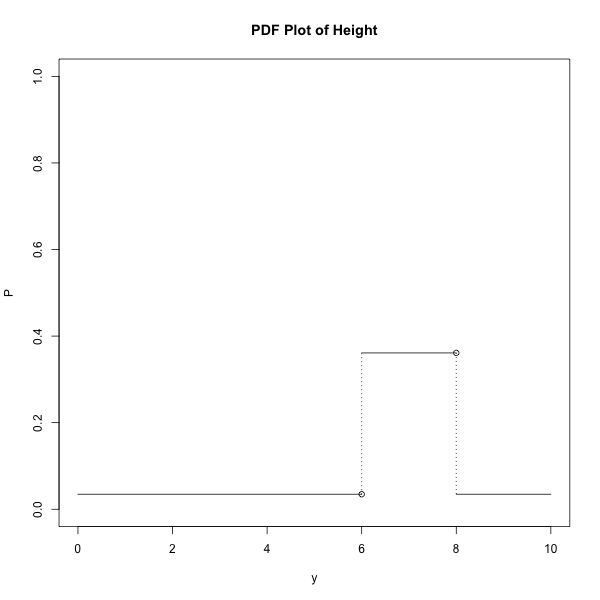
\includegraphics[height= 3in]{Q1_pdf.png}\\
\end{center}
(c) Let event A be that the spider is located outside the painting area.\\
 $F_{X,Y|A} = \frac{p(X\leq x,Y\leq y,A)}{P(A)}$, $P(A) = \frac{1}{3}$\\
For $y \in [0,6], F(Y) = P(Y \in [0,y]) = \int_{0}^{y} \int_{0}^{10}  3f_{X,Y,A}{(u,v)} du dv =  \int_{0}^{y} \int_{0}^{10}  \frac{3}{288}dudv = \frac{30}{288} y$,\\
For $y \in [6,8],F(Y) = P(Y \in [6,y])+P(Y\in [0,6]) = \int_{6}^{y} \int_{0}^{10}  f_{X,Y,A}{(u,v)} du dv + \frac{180}{288}$\\
$  \int_{6}^{y} \int_{0}^{10}  f_{X,Y,A}{(u,v)} du dv =  \int_{6}^{y} \int_{0}^{4} 3\frac{1}{288} du dv + \int_{6}^{y} \int_{6}^{10} 3\frac{1}{288} du dv = \frac{24}{288}(y-6) $\\
For $y \in [8,10], F(Y) = P(Y \in [0,8])+P(Y \in [8,y])  = \int_{8}^{y} \int_{0}^{10}  f_{X,Y,A}{(u,v)} du dv + \frac{228}{288}=  \frac{228}{288} +\int_{8}^{y} \int_{0}^{10}  3\frac{1}{288}dudv =  \frac{30}{288} (y - 8) + \frac{228}{288}$\\
%Therefore, the pdf is $\frac{30}{288}$ for y $\in [0,6]  \bigcup [8,10]$, $\frac{24}{288}$ for y $\in [6,8]$
 \begin{center}
 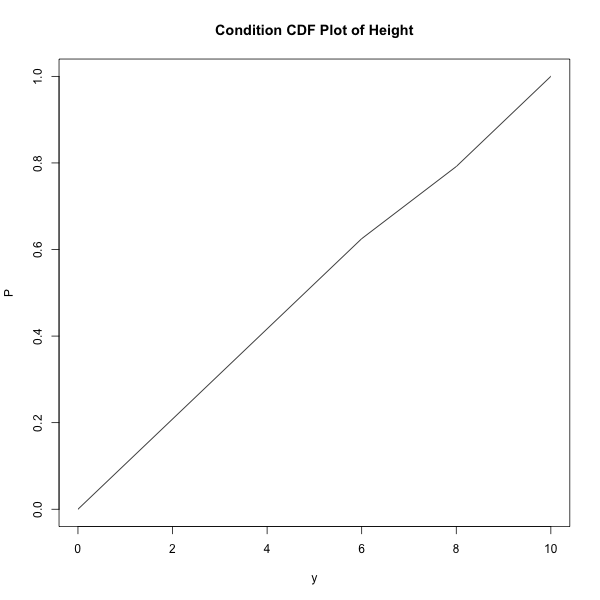
\includegraphics[height = 4in]{Q1_2}\\
 \end{center}
 
 \begin{problem}{2}
\end{problem}
(a) Let X be the time until Pat receives a call, Y be the time until Robbie receives a call. If we assume that the customer has no preference between the two restaurant and order pizzas independently, let the time until one of them receives a call be $T_1$. $P(0<T_1<t) = 1- P(X>t , Y>t)$\\
Since X,Y are independent by assumption, $P(X>t , Y>t) = P(X>t) \times P(Y>t) = \int_{t}^{\infty} \lambda e^{-\lambda x}dx  \int_{t}^{\infty} \lambda e^{-\lambda y}dy = (-e^{-\lambda x}|_t^\infty)^2 = e^{-2\lambda t}$\\
$P(0<T_1<t) = 1 - P(X>t , Y>t)  = 1 - e^{-2\lambda t }$\\

(b) Making the same assumption as part (a),  let $T_2$ be the time until both of them have received a call. If both of them received the call until t, the possibility should be X received at any time within [0,t], and Y received at any time within [x,t] as well as the symmetric case of Y received first.\\
$P(T_2<t) = 2 \times \int_{0}^{t} \int_{x}^{t}\lambda e^{-\lambda x} \lambda e^{-\lambda y}dydx = 2\int_{0}^{t} \lambda e^{-\lambda x} (-e^{-\lambda y}|_x^t)dx = 2\int_{0}^{t} \lambda e^{-2\lambda x} - \lambda e^{-\lambda t } e^{-\lambda x}dx$\\
$ = 2(-\frac{e^{-2\lambda x}}{2}|_0^t + e^{-\lambda t} e^{-\lambda x}|_0^t) = e^{-2\lambda t} - 2e^{-\lambda t} +1$\\

(c)The result is reasonable. Let the individual waiting time distribution be $T_3$. At any given time, the probability of at least one of  them receive a call should be greater than that of both of them receive a call. The corresponding CDF plots are identical to this fact, in particular $T_1$ lies above $T_2$. The event Pat receives a call at time t is contained in the event that at least one of them receive a call. Meanwhile, it contain the event that both of them receive call. In the plot we observed that $T_2(t)<T_3(t) < T_1(t),\forall t >0$, this is identical to the fact. \\
\begin{center}
	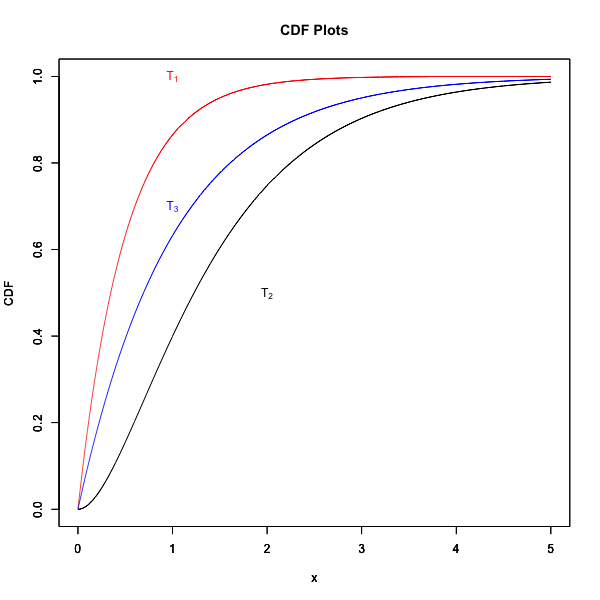
\includegraphics[height = 3.8in]{Q2_3}
  \end{center}

\newpage

\begin{problem}{3}
	\end{problem}
(a) Let X be a Binomial(n,$\frac{1}{2}$), and $X_k$ be the events that X = k. Since $X_i 's$ are disjoint events and $\bigcup X_k$ is the whole sample space defined by X. By the axiom of probability: $P(\bigcup_{k=0}^n X_k) = \sum_{k =0}^{n}P(X_k) =  1$\\
$\sum_{k =0}^{n}P(X_k) = \sum_{k =0}^{n} {n \choose k}(\frac{1}{2})^k (\frac{1}{2})^{n-k} =\frac{\sum_{k =0}^{n} {n \choose k}}{2^n}  = 1$\\
Therefore, $\sum_{k =0}^{n} {n \choose k} = 2^n$\\

(b)Let N be the number of mechanical problem that the two people will encounter per month. We assume that the cars encounter problems independently.\\
$P(N = n) = \sum_{k =0}^{n} \frac{\lambda^k}{k!}e^{-\lambda} \frac{\lambda^{n-k}}{(n-k)!}e^{-\lambda}  =  e^{-2\lambda} \sum_{k =0}^{n} \frac{\lambda^n}{k!(n-k)!} =e^{-2\lambda} \frac{\lambda^n}{n!}\sum_{k =0}^{n} \frac{n!}{k!(n-k)!}  = e^{-2\lambda} \frac{\lambda^n}{n!} 2^n = e^{-2\lambda} \frac{(2\lambda)^n}{n!}$\\

\begin{problem}{4}
\end{problem}
(a) Let X, Y be the positions of Mary and Hannah respectively. They are independently and  uniformly distributed over [0,10]$\times [0,10]$. The joint pdf $f_{X,Y} = \frac{1}{100}$ for $(X,Y) \in  [0,10] \times [0,10] $ and 0 otherwise.
\begin{center}
	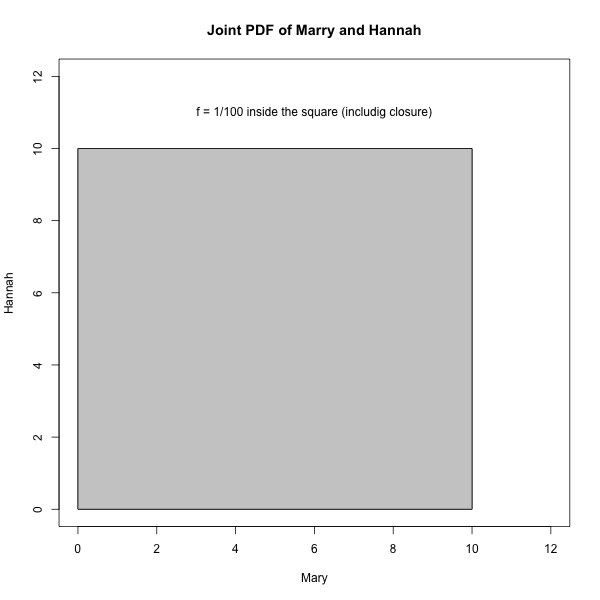
\includegraphics[height = 4in]{Q4_1}
	\end{center}

\newpage

(b)\begin{center}
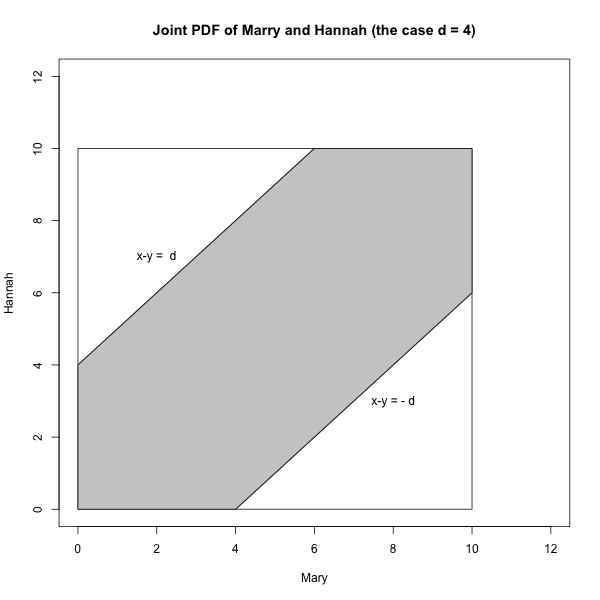
\includegraphics[height = 3.2in]{Q4_2}
\end{center}
 
 
 (c)  Let the distance be D. $P(D \in [0,d]) $ is just the percentage of the shaded region for any give d.
 $P(D \in [0,d])  = \frac{100 - (10-d)^2}{100} = \frac{20d - d^2}{100}$\\
 the pdf is $ f (d)= \frac{20 - 2d}{100}$
 \begin{center}
 	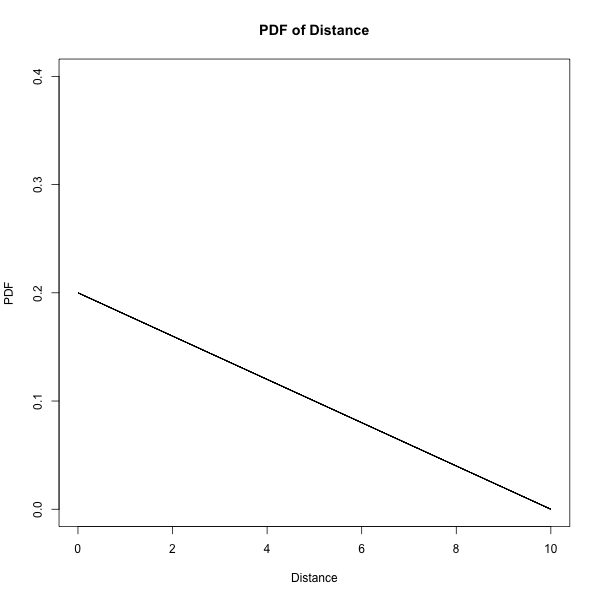
\includegraphics[height = 3in]{Q4_3}
 \end{center}
 
 \begin{problem}{5}
 \end{problem}
  (a) Let C be the bias of the coin, C $\sim $ Unif($\frac{1}{2}$,1), and D be the outcome of the coin flip. The parameter of the distribution of outcome depends on the bias. In Particular,   $P(D = heads|C = c ) = c $\\
  $P(D = heads) = \int_{0.5}^{1} P(D = heads| C = c ) f(c)dc = \int^{1}_{0.5} c \times 2 dc = 1- \frac{1}{4} = \frac{3}{4}$\\
  $P(D = tails ) = \frac{1}{4}$\\
  
  (b) $f(c|D = heads) = \frac{f_c(c) P_{D|C}(D = heads| C =c)}{P_D(D = heads)} = \frac{2 c}{3/4 } = \frac{8c}{3}$\\
  $ f(c|D = tails) = \frac{f_c(c) P_{D|C}(D = tailss| C =c)}{P_D(D = tails)} = \frac{2 (1-c)}{1/4 } = 8(1-c)$\\
  The posterior of bias given getting a head is $\frac{8c}{3}$, Thus the cdf is $\frac{8}{6} c^2 -\frac{1}{3}, 0.5 \leq c \leq 1  $\\
  The posterior of bias given getting a tail is $8-8c$, Thus the cdf is $8c - 4c^2 -3, 0.5 \leq c \leq 1  $\\ 
  
  If we continue the flip:\\
  i) For D = heads, $f_{i+1}(c|D = heads) = \frac{f_{c,i}(c) P_{D|C}(D = heads| C =c)}{P_D(D = heads)}  = \frac{f_{c,i}(c) c}{\int_{0.5}^{1} c f_{c,i}(c)dc}$\\
  %$f_{c,i} $ is a polynomial with degree i, i.e $constant \times c^i$\\ Therefore $f_{i+1}(c|D = heads) = \frac{c^{i+1}}{\frac{c^{i+2}}{i+2}|_{0.5}^1} = \frac{(i+2)c^{i+1}}{1- 0.5^{i+2}}, i = 0,1,2,...$ \\
  %The CDF is $\frac{1}{1-0.5^{i+2}} (c^{i+2} - 0.5^{i+2}), i =0,1,2,...$\\
  ii) For D = tails, $ f_{i+1}(c|D = tails) = \frac{f_{c,i}(c) P_{D|, i = C}(D = tailss| C =c)}{P_D(D = tails)} = \frac{f_{c,i}(c)(1-c)}{\int_{0.5}^{1} f_{c,i}(c)(1-c)dc} $\\
  %= \frac{(1-c)^{i+1}}{\frac{(1-c)^{i+2}}{i+2}|_{0.5}^1} = \frac{(i+2)(1-c)^{i+1}}{(0.5)^{i+2}}, i = 0, 1,2,...$\\
  %The CDF is $(-1)^{i+1} 2^{i+2}({(1 - c)^{i+2} - 0.5^{i+2}}) = (-1)^{i+1}( (2-2c)^{i+2}-1), i = 0,1,2,...$   
    
  \begin{center}
  	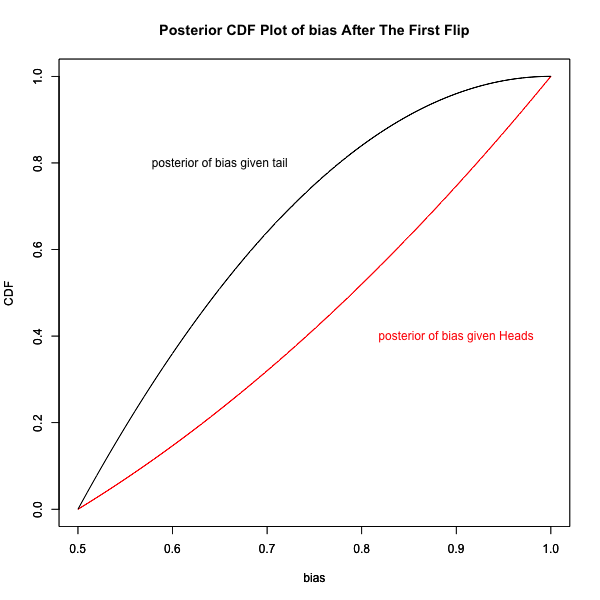
\includegraphics[height = 4in]{Q5_2}
  \end{center}
  This is reasonable, because if a head is observed the bias is more likely to be distributed close to 1.Therefore the CDF of the posterior is convex. If a tail is observed, the bias is more likely to be distributed close to 0.5. Thus the CDF is concave.    
  
  
  
 
\end{document}